\section{Deskriptive Analyse}

\begin{frame}\frametitle{Inhalt}
	\tableofcontents[currentsection,hideallsubsections]
\end{frame}

\begin{frame}\frametitle{Beispiel für einen Auszug aus der Datenbank}
	\begin{table}[H]
		\begin{center}
			\begin{tabular}{|c|l|c|c|c|c|}
				\hline
				ID & Campaign 									 & Transaction & Position & ... \\ \hline\hline
				1  & Affiliate - Partnerprogramm & 0					 & 1		    & ... \\ \hline
				1  & SEM - Brand                 & 0					 & 2		    & ... \\ \hline
				1  & Direct                      & 0					 & 3		    & ... \\ \hline
				1  & Direct                      & 1					 & 4		    & ... \\ \hline
				2  & Display                     & 0					 & 1		    & ... \\ \hline
				2  & SEM - Generisch             & 0					 & 2		    & ... \\ \hline
				2  & Social Media                & 0					 & 3		    & ... \\ \hline
			\end{tabular} 
		\end{center}
	\end{table}
\end{frame}

\begin{frame}\frametitle{Datenlage} 
	\begin{itemize}
		\item SQL-Dump mit Größe von circa $13$ Gigabyte
		\item Einteilung in konvertierte und nicht-konvertierte Funnels
		\item Kampagnen in Form einer Baumstruktur organisiert
		\item Festlegung auf $17$ Kategorien
		\item \textit{Views} liegen in den nicht-konvertierten Funnels nur vor, wenn diese bei einem anderen Kunden der Refined Labs GmbH konvertiert sind
		\item $ 297,963 $ \textit{Clicks} für die konvertierten und $ 9,550,802 $ \textit{Clicks} für die nicht-konvertierten Funnels
		\item Erstellung von Features
	\end{itemize}
\end{frame}

\subsection{Views in den konvertierten Funnels}

\begin{frame}\frametitle{clickCount}
	    \centering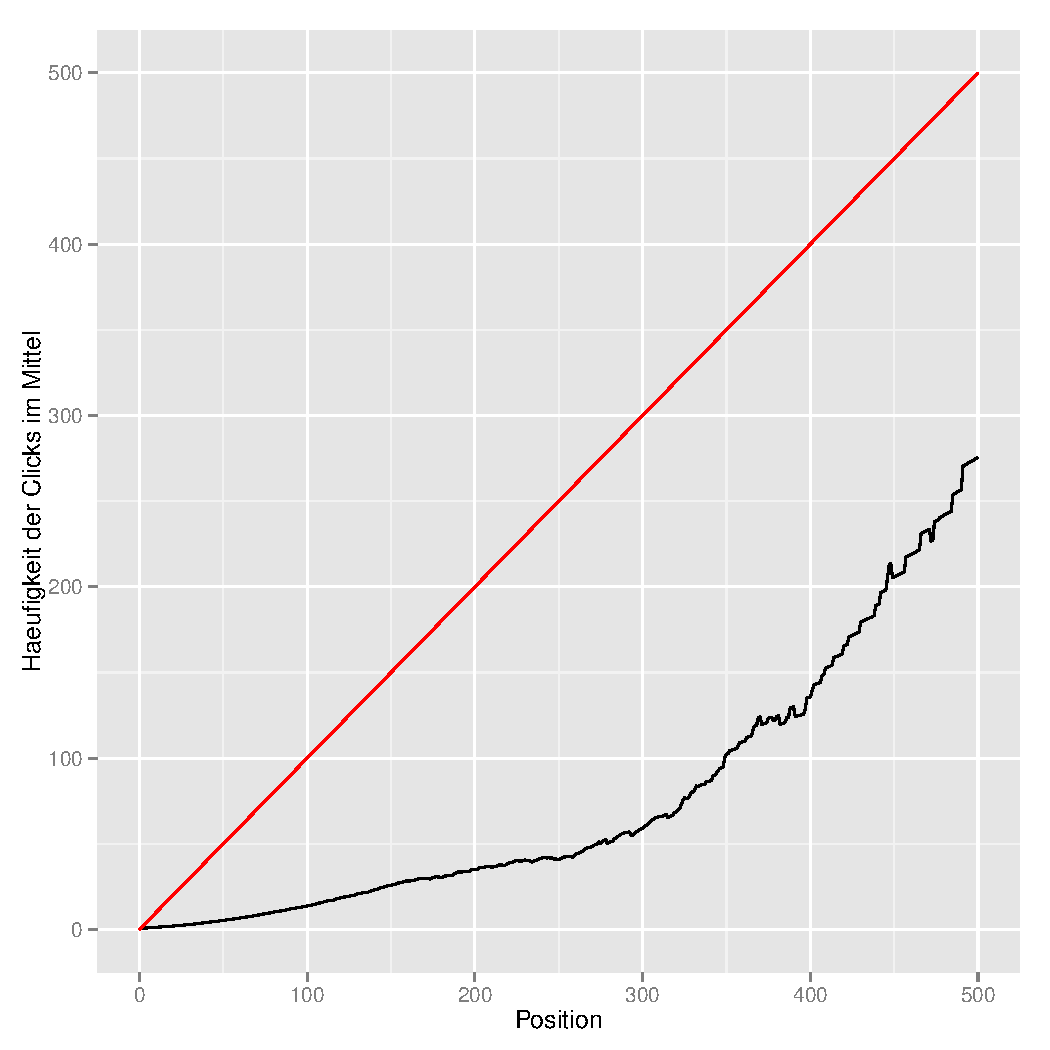
\includegraphics[scale=0.39]{clickCountSucc.pdf}
\end{frame}

\begin{frame}\frametitle{hasClicked}
	    \centering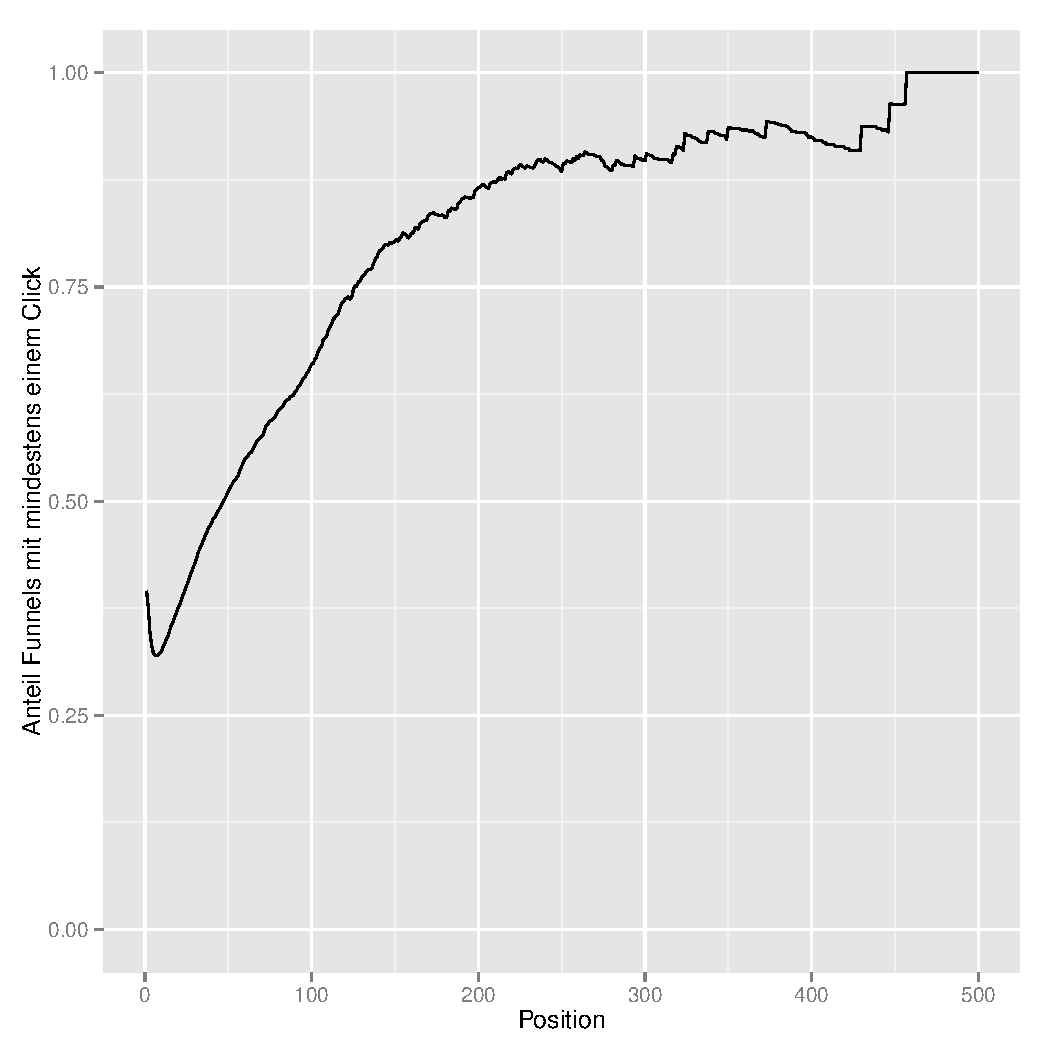
\includegraphics[scale=0.39]{hasClickedSucc.pdf}
\end{frame}

\begin{frame}\frametitle{Beschreibung der Kampagnen}
	\begin{table}[H]
		\tiny
		\begin{center}
			\begin{tabular}{|l|p{7cm}|}
				\hline \textbf{Kampagne} & \textbf{Beschreibung}\\ \hline
				\hline Affiliate - Partnerprogramm & Partner, die von der Interhyp AG bereitgestellte Werbemittel wie Rechner, Logo oder Banner einbinden\\
				\hline Affiliate - Rest & Partner, die einen Zinsvergleich bereitstellen, welcher das Zinsangebot der Interhyp AG mit deren Wettbewerbern im Vergleich darstellt\\ 
				\hline Direct & Potentieller Kunde gibt im Browser direkt \textit{www.interhyp.de} ein\\ 
				\hline Display & Bannerschaltungen\\
				\hline E-Mailing & Mails an Interessenten, die schon einen Antrag gestellt oder ein Infopaket angefordert hatten\\
				\hline Generic & Potentieller Kunde kommt über unbezahlten Link zur Interhyp AG\\
				\hline Kooperationen - Focus & \multirow{5}{7cm}{Individuelle Zusammenarbeiten mit größeren Partnern, die je nach Vertrag verschiedene Werbemittel auf ihrer Seite einbinden}\\
				Kooperationen - Immonet & \\
				Kooperationen - Immoscout24 & \\
				Kooperationen - Immowelt & \\
				Kooperationen - Rest & \\
				\hline Newsletter & Regelmäßige Rundschreiben\\
				\hline SEM - Brand & Bezahlte Suchergebnisse, wobei nach \textit{Interhyp} oder ähnlichem gesucht wurde\\
				\hline SEM - Remarketing & Bezahlte Suchergebnisse, wobei der potentielle Kunde bereits zuvor auf der Seite der Interhyp AG war\\
				\hline SEM - Generisch & Bezahlte Suchergebnisse, wobei nach \textit{Baufinanzierung} oder ähnlichem gesucht wurde\\
				\hline SEO & Unbezahlte Suchergebnisse\\
				\hline Social Media & Werbung, vor allem auf \textit{facebook} und \textit{gutefrage.net}\\
				\hline
			\end{tabular} 
		\end{center}
	\end{table}
\end{frame}

\begin{frame}\frametitle{campaign}
	    \centering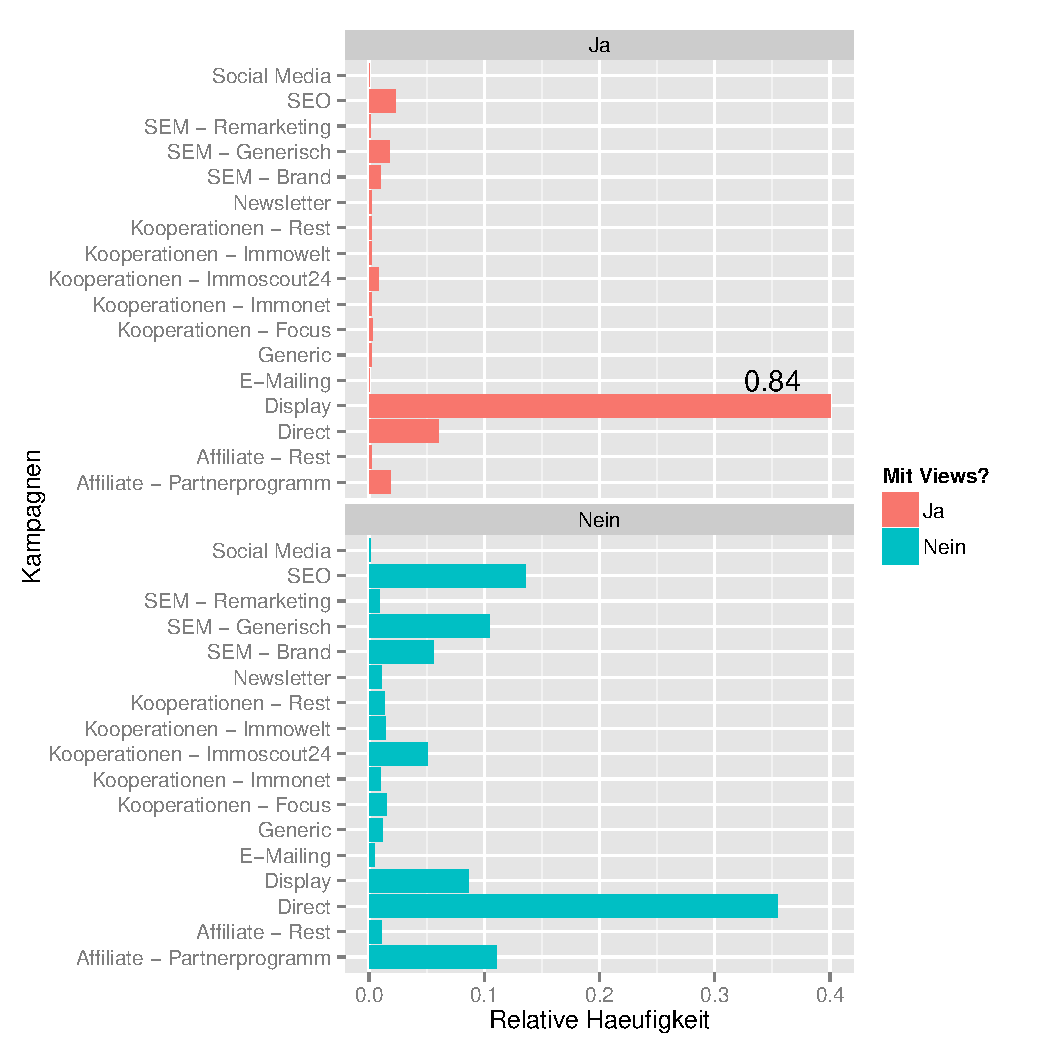
\includegraphics[scale=0.3]{campaignSucc.pdf}
\end{frame}

\subsection{Vergleich von konvertierten und nicht-konvertierten Funnels}

\begin{frame}\frametitle{weekday}
	    \centering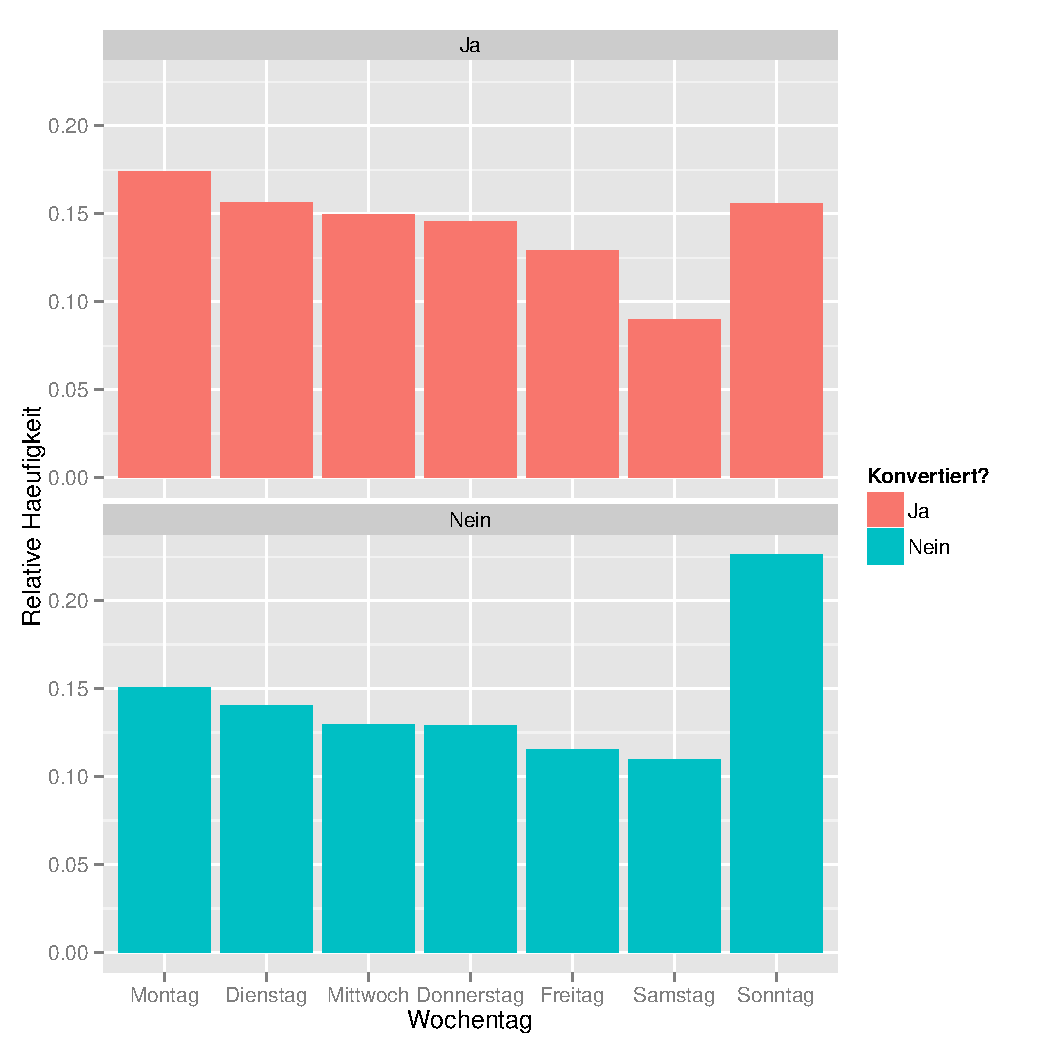
\includegraphics[scale=0.3]{weekday.pdf}
\end{frame}

\begin{frame}\frametitle{hour}
	    \centering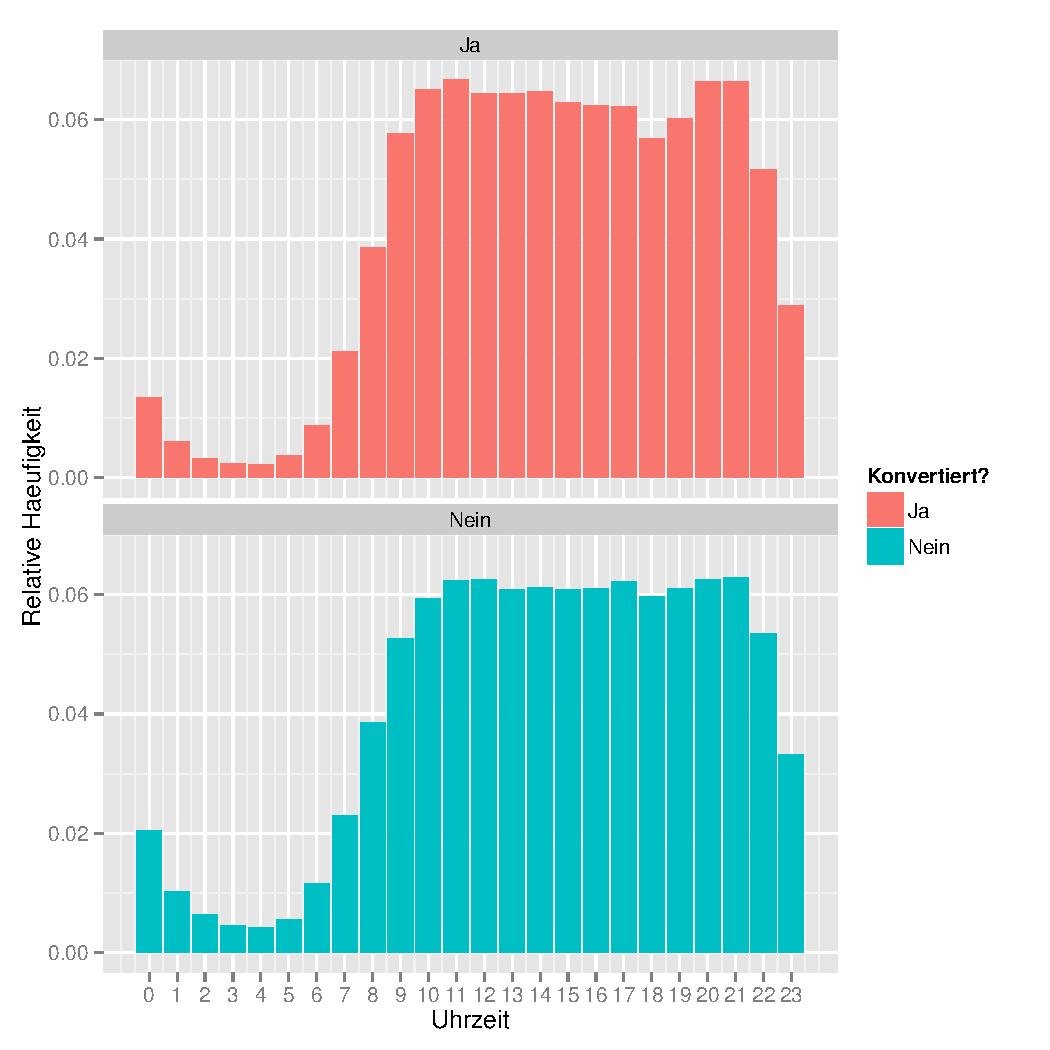
\includegraphics[scale=0.3]{hour.pdf}
\end{frame}

\begin{frame}\frametitle{campaign}
	    \centering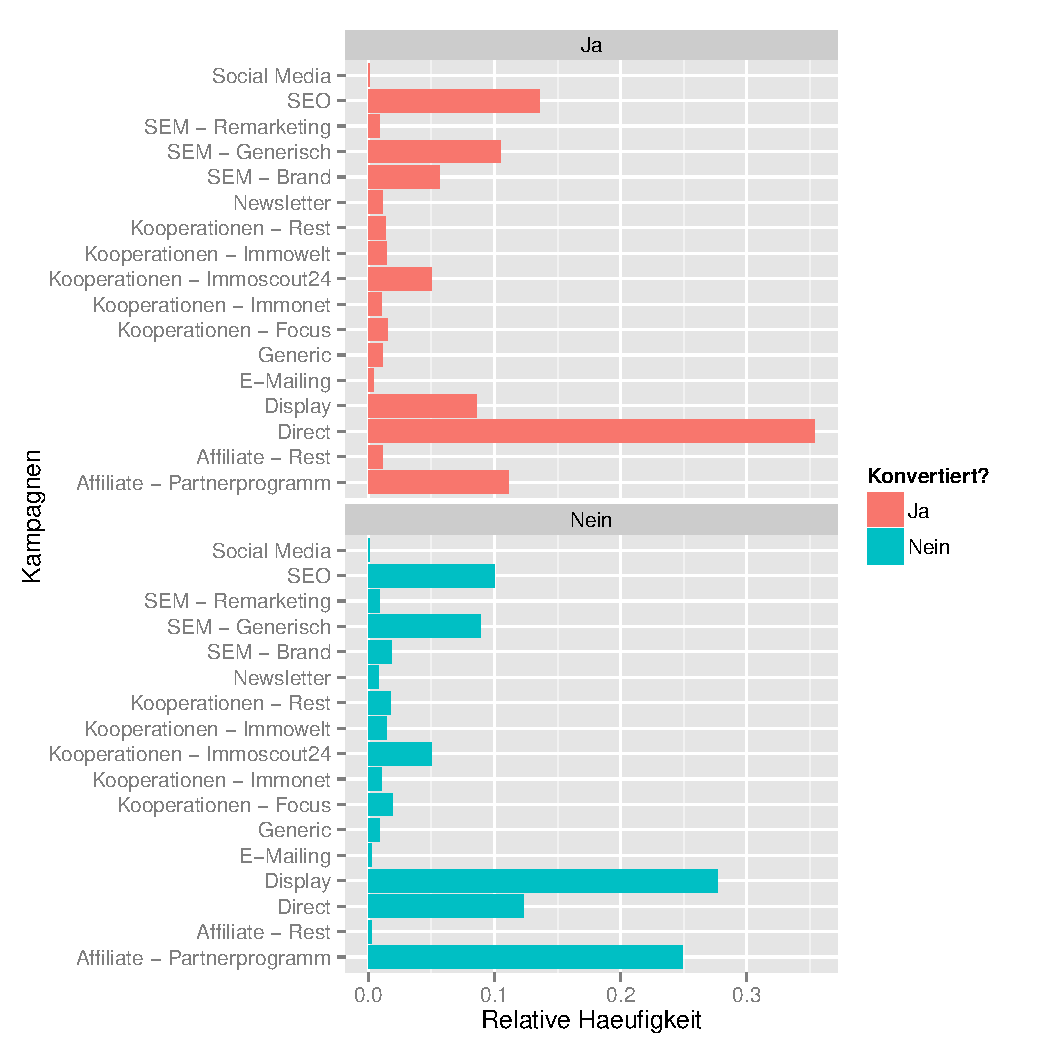
\includegraphics[scale=0.3]{campaign.pdf}
\end{frame}

\begin{frame}\frametitle{funnelLength}
	    \centering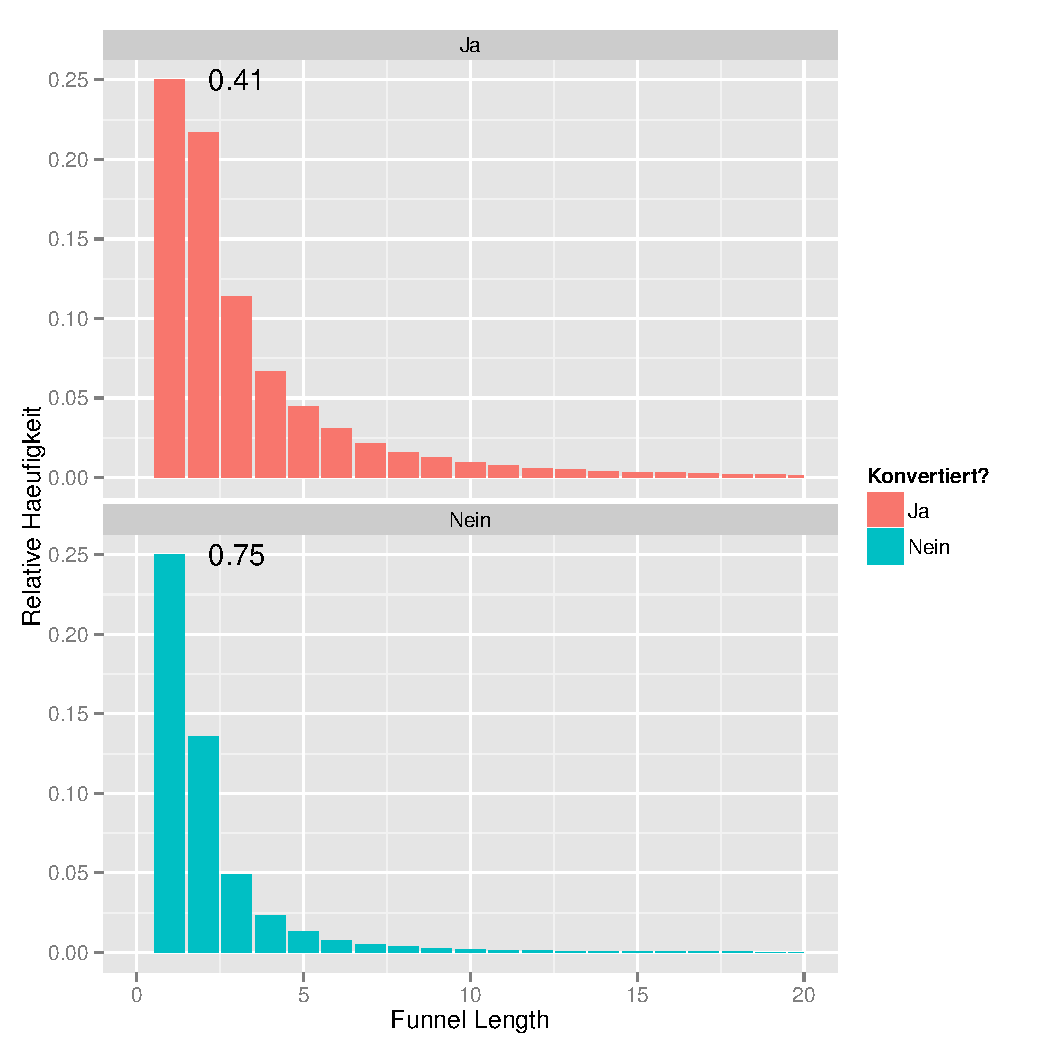
\includegraphics[scale=0.3]{funnelLength_First.pdf}
\end{frame}

\begin{frame}\frametitle{timeSinceFirst}
	    \centering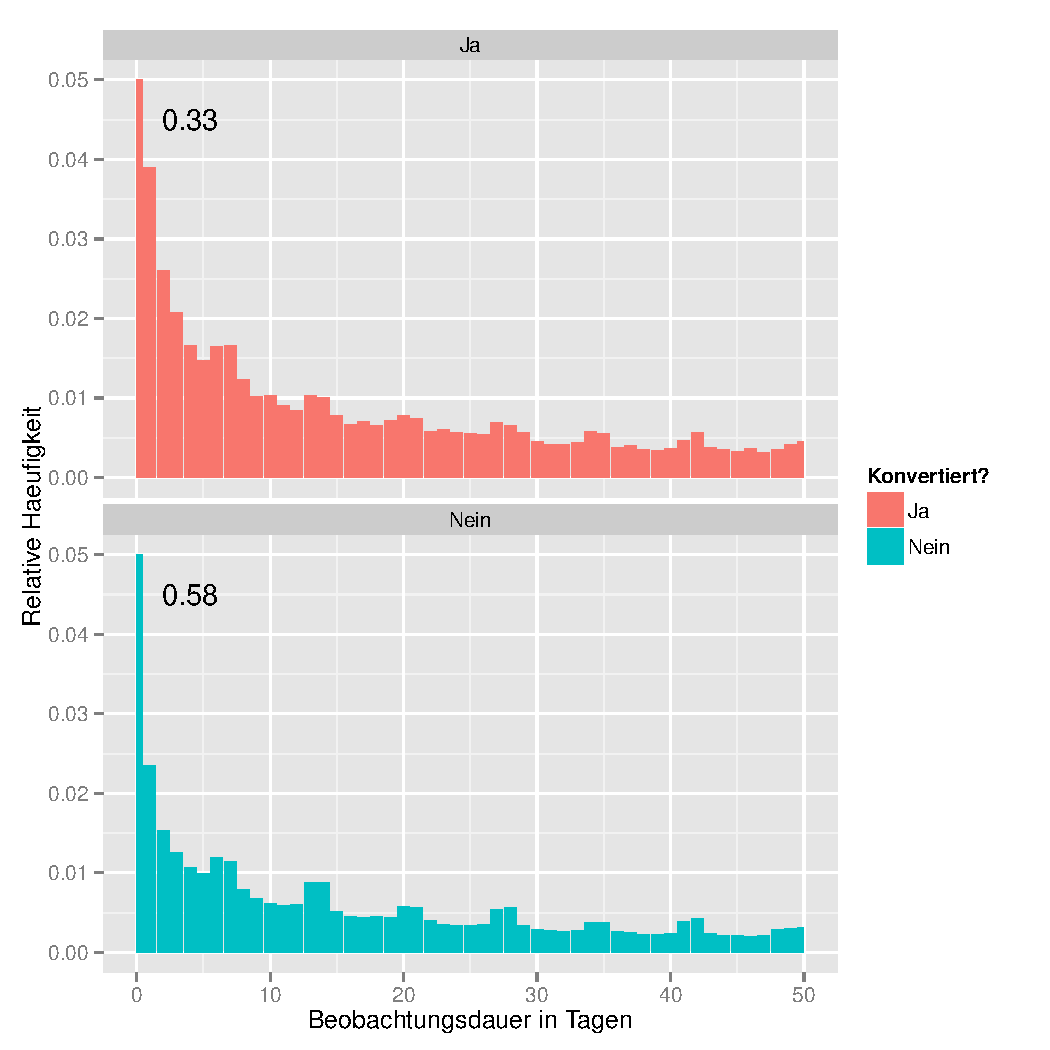
\includegraphics[scale=0.3]{timeSinceFirst_Last.pdf}
\end{frame}

\begin{frame}\frametitle{timeSinceLast}
	    \centering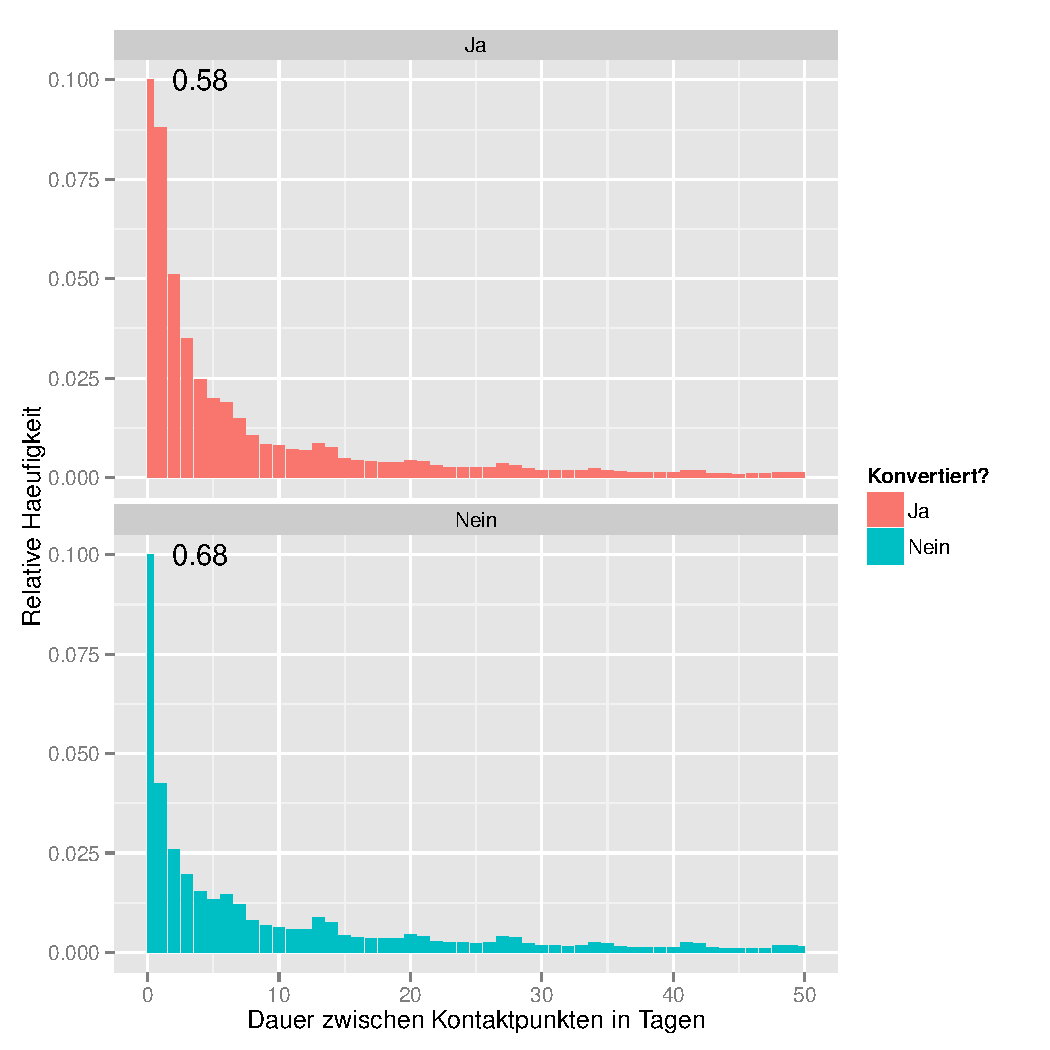
\includegraphics[scale=0.3]{timeSinceLast.pdf}
\end{frame}

\begin{frame}\frametitle{freq}
	    \centering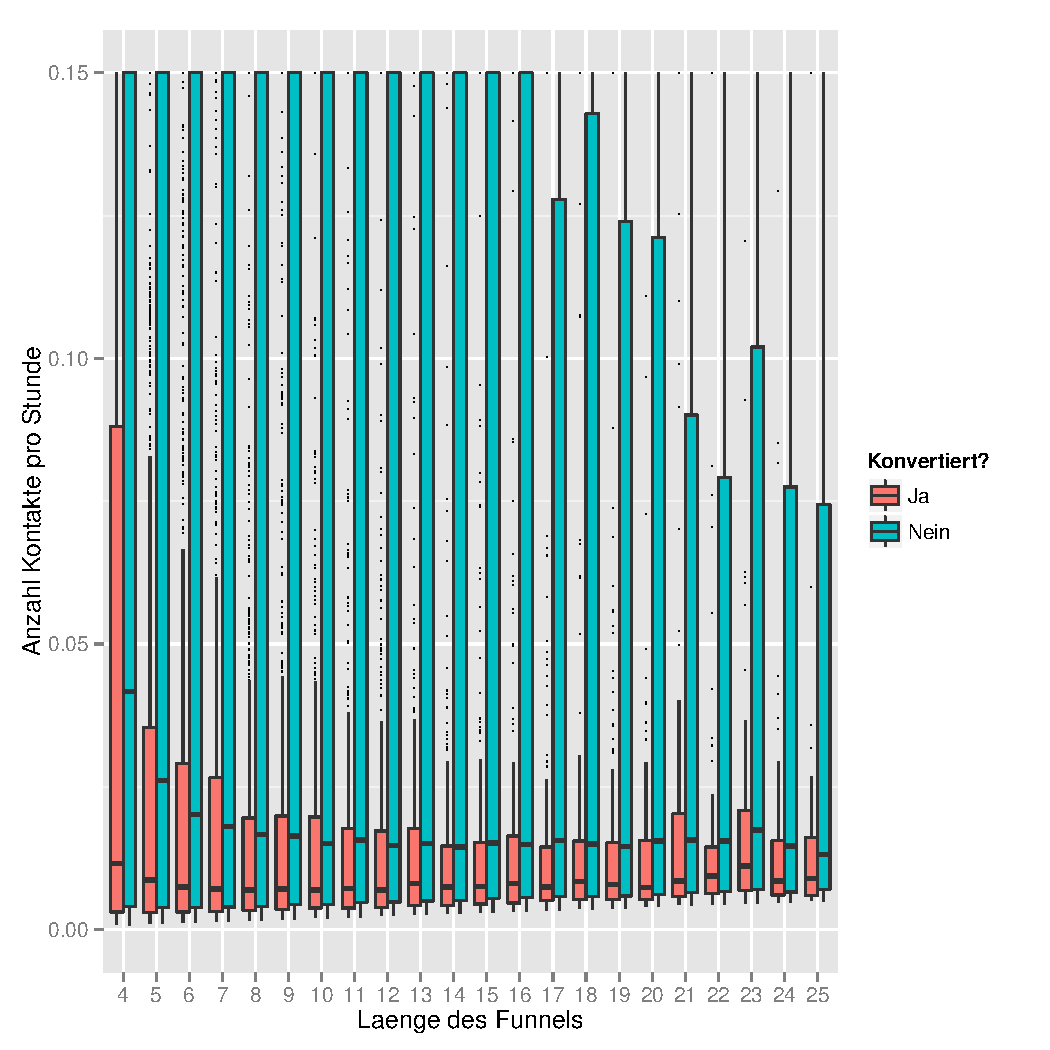
\includegraphics[scale=0.3]{freq.pdf}
\end{frame}
